\documentclass{llncs}

\usepackage{subfigure}
\usepackage{epsfig}
\usepackage{color}
%\usepackage{balance}
\usepackage{paralist}
\usepackage{pdfsync}
\usepackage{makeidx}  % allows for indexgeneration

\begin{document}

\pagestyle{headings}

\newif\ifdraft
%\drafttrue
\ifdraft
\newcommand{\kimnote}[1]{ {\textcolor{green} { ***JK: #1 }}}
\newcommand{\alnote}[1]{ {\textcolor{blue} { ***AL: #1 }}}
\newcommand{\amnote}[1]{ {\textcolor{magenta} { ***AM: #1 }}}
\newcommand{\jhanote}[1]{ {\textcolor{red} { ***SJ: #1 }}}
\else
\newcommand{\kimnote}[1]{}
\newcommand{\alnote}[1]{}
\newcommand{\amnote}[1]{}
\newcommand{\jhanote}[1]{}
\fi

% \newcommand{\up}{\vspace*{-1em}}
% \newcommand{\upp}{\vspace*{-0.5em}}
\newcommand{\up}{\vspace*{0em}}
\newcommand{\upp}{\vspace*{0em}}



\title{ ~\\[-3em] Developing Scientific Applications With
  Loosely-Coupled Sub-Tasks}

\author{Shantenu Jha, Yaakoub El-Khamra, Joohyun Kim}

\institute{Center for Computation and Technology, Louisiana State
  University, Baton Rouge LA 70803, USA} % \and
%Department of Computer Science, Louisiana State University, Baton Rouge LA 70803, USA \and
%Institute of Computer Science, Potsdam University, Germany}

\maketitle

\newenvironment{acknowledgement}%

{\section*{\acknowledgementname}%
\parindent=0pt%
}

% \begin{abstract}
%   The Simple API for Grid Applications (SAGA) can be used to
%   programmatically develop a very wide-range of distributed
%   applications.  In this paper we describe how SAGA has been used to
%   develop two different applications from the following classes of
%   distributed applications (i) applications based upon the loose
%   coupling of homogenous sub-tasks and, (ii) applications based upon
%   loose coupling of simulations of heterogenous sub-tasks.  The nature
%   of the coupling also varies significantly for these applications,
%   and plays an important role in the development and deployment
%   options available.  The specific applications developed are
%   Replica-Exchange simulations using Molecular Dynamics and
%   Kalman-Filter based application for reservoir simulation.  We
%   briefly discuss the specific applications developed and the typical
%   science problems tackled using these applications.  We will describe
%   the application characteristics of the two case-studies, with a
%   focus on the distributed logic of these simulations, and not the
%   core simulation logic of the applications.  The paper analyses and
%   contrasts the application characteristics of the examples, and shows
%   how they are supported using SAGA, often in conjunction with other
%   programming frameworks such as Cactus. Along with the development of
%   multi-task applications, it is also important to focus on the
%   deployment challenges, especially if, as we will argue that the
%   dynamic applications (which form an important class of applications
%   with multi-tasks) in addition to requiring programming models tht
%   support explicit distributed, must also have an agile execution
%   model.  The primary aim of this paper is to demonstrate how SAGA can
%   be an effective tool for programmatically representing and
%   implementing the logic of coordination and orchestrating multiple,
%   distributed tasks, while remaining agnostic to the actual mechanism,
%   ie. details of the distributed environment. We will highlight the
%   importance of programming abstractions and how frameworks that
%   provide common programming patterns can be used to simplify the
%   construction of distributed applications.
% \end{abstract}


\begin{abstract}
%  The aim of this paper is to demonstrate how 
  The Simple API for Grid Applications (SAGA) can be used to develop a
  range of applications which are in turn composed of multiple
  sub-tasks.
  %with agile execution models. 
  In particular SAGA is an effective tool for coordinating and
  orchestrating the many sub-tasks of such applications, whilst
  keeping the application agnostic to the details of the
  infrastructure used. Although developed primarily in the context of
  distributed applications, SAGA provides an equally valid approach
  for applications with many sub-tasks on single high-end
  supercomputers, such as emerging peta-scale computers.
  % dynamic applications with many sub-tasks,
  %possibly distributed, 
  Specifically, in this paper we describe how SAGA has been used to
  develop applications from two types of applications: the first with
  loosely-coupled homogeneous sub-tasks and, applications with
  loosely-coupled heterogeneous sub-tasks. We also analyse and
  contrast the coupling and scheduling requirements of the sub-tasks
  for these two applications.  We find that applications with multiple
  sub-tasks often have dynamic characteristics, and thus require
  support for both infrastructure-independent programming models and
  agile execution models. Hence attention must be paid to the
  practical deployment challenges along with the theoretical advances
  in the development of infrastructure-independent applications.
\end{abstract}

\section{Introduction}
There exist many scientific problems that are solved by the collective
analysis of many independent tasks, e.g., Monte-Carlo simulations, or
parameter sweeps.  There also exists a large class of scientific
problems that involve applications that can either be decomposed into
smaller coupled sub-tasks via the of choice an appropriate
algorithm~\cite{spice_sc05}, or are naturally composed of coupled
sub-tasks. The decomposition of an otherwise monolithic application
into smaller components of computation, in principle makes them
amenable to efficient distribution. 

In this paper, we discuss Replica-Exchange (RE) and Ensemble
Kalman-Filter (EnKF) based applications, as representative prototypes
of applications with coupled sub-tasks.  Although similar at some
levels, they possess important differences.  For RE based
simulations, the sub-tasks are identical (ie. replicas), whereas for
the EnKF the sub-tasks are heterogeneous. Additionally the nature of
coupling between the sub-tasks in the former (regular intervals and
pair-wise) is very different from the latter (irregular and a
global-synchronisation point).

It is important to appreciate the difference between
loosely-coupled when typically used in the context of parallel
applications versus when used in the context of distributed
applications. For the former, loosely-coupling is most often a
reference to the application's tolerance of latency in message
passing. For distributed applications loose (or tight) coupling has
more context: it could be a reference to the flexibility in scheduling
and placing the sub-tasks or even a flexibility in choice of resources
the different sub-tasks are mapped to. Although both applications we
investigate are classified as loosely-coupled, the nature of the
coupling between their sub-tasks varies. It is important to appreciate
The nature of the coupling of the sub-tasks, in addition to imposing
constraints on scheduling and resource mapping strategies, also
determines the feasibility of any speculative computing.  Thus, along
with the size and number of sub-tasks, the nature of coupling
determines the overall development and deployment strategy.

% In the latter case, they are not only heterogeneous they are also
% highly irregular and both applications need to be adaptive to dynamic
% changes in order to function effectively.

% loosely-coupled identical sub-tasks (ie replicas) and loosely-coupled
% but heterogenous sub-tasks.

In addition to some similarity between application characteristics,
what binds the two together, is our adopted approach of developing
distributed applications. The Simple API for Grid Applications
(SAGA)~\cite{saga_url} provides a simple, standard, programmatic
approach to codify distributed applications such that they can be
seamlessly run on any underlying infrastructure. Critically, this
allows the application developer to focus on supporting the
application characteristics and exploiting the relative strengths of
different infrastructure whilst not worrying about adapting to the
details of the infrastructure. Not being coupled to the
details of the underlying infrastructure is a necessary condition for
applications whose resource requirement might increase or those that
want to make opportunistic use of newly available resources. In
other words independence from specific infrastructure, is a necessary
condition for dynamic applications to achieve the desired
agile-execution models and thus be adaptive.  The aim of this paper is
to discuss how SAGA has been used to develop two applications with
multiple sub-tasks in a way such that these applications can be
deployed and executed on both distributed as well high-end machines,
with a minimal, if not no-changes.

% We posit that along with the size and number of sub-tasks,
% the coupling between the sub-tasks is an important determinant of the
% development and deployment mechanism.

% In the former, the sub-tasks progress independent of other sub-tasks
% with the exception of one (referred to as the paired replica). There
% is a pair-wise exchange of some parameters after a certain time-period
% (maybe fixed or not), and it is possible that the paired-replicas
% differ, i.e., a replica is paired with a different replica as time
% progresses. If the sub-task that a replica is paired with is not is
% not ready for exchange, the sub-tasks goes into a wait state, i.e.,
% the consequence of load-balancing is typically localized to the paired
% replica. If there are multiple replicas in a wait state, sophisticated
% scheduling can be invoked to progress waiting
% tasks. \jhanote{elaborate a bit}

% It is important to contrast this ``coupling'' with the coupling in the
% latter application's (EnKF) case. For the EnKF application, the
% multiple sub-tasks need to {\it all} complete as there is a global
% synchronization point, and the output of all sub-tasks are required to
% generate the input for the next stage.

% As we will go onto discuss, using general purpose grid
% infrastructure Our experiences are consistent with the fact that it
% is ~\cite{TeraGyroid}

Lingering problems associated with deployment on production Grids
% general-purpose Grids %(ie broad-Grids) 
has made the uptake of Grids challenging and unattractive to the end-scientist. In a
nutshell, our experience is consistent with and indicates that one of
the reasons deployment on general-purpose Grids is difficult, because
Grids are comprised of many ``isolated'' components. We believe
that this contributes to a currently unmanageable number
degrees-of-freedom and failure modes.  %Thus, 
Although programming models and conceptual frameworks exists to unify the uptake of ``grids
or supercomputers'' as required, practical considerations make this
currently unrealistic and motivate the end-scientist to settle for the
the solution that is often simpler to deploy. Whereas this has
consequences for all distributed applications, it influences the
development and uptake of {\it dynamic} distributed applications.
% particularly.  
Although the focus here is on utilising distributed
%multiple 
machines, the same approach can be used for monolithic large
machines. We demonstrate the validity of the SAGA approach for
high-performance computing on large single machines.

% , of which there are a large number of multiple sub-task
% applications.

% \jhanote{The bulk of the next three sections should be pretty much a
%   cut and paste job. What is really required is i. run the multi-tasks
%   of the Kalman filter application entirely on Abe ii. run the
%   multi-tasks of the replica exchange entirely on Abe}

\jhanote{Although they belong to different classes, we show here that
  they can be deployed effectively on i) Range of systems and scales,
  a smaller but many distributed systems as well as a single, but much
  larger top-end system. ii) Explicitly versus Implicitly: dynamic
  applications profit from being able to have.....}

\section{SAGA: A Standard Programming Interface}

The Simple API for Grid Applications (SAGA) is an API standardization
effort within the Open Grid Forum (OGF)~\cite{ogf_web} an
international standards development body concerned primarily with
standards for distributed computing.  SAGA provides a simple,
POSIX-style API to the most common Grid functions at a sufficiently
high-level of abstraction so as to be able to be independent of the
diverse and dynamic Grid environments.  The SAGA specification defines
interfaces for the most common Grid-programming functions grouped as a
set of functional packages.  The SAGA Version 1.0 specification
defines the following packages:

\begin{figure}[!h]
  \begin{center}
    \subfigure{\label{sagalayer1}
      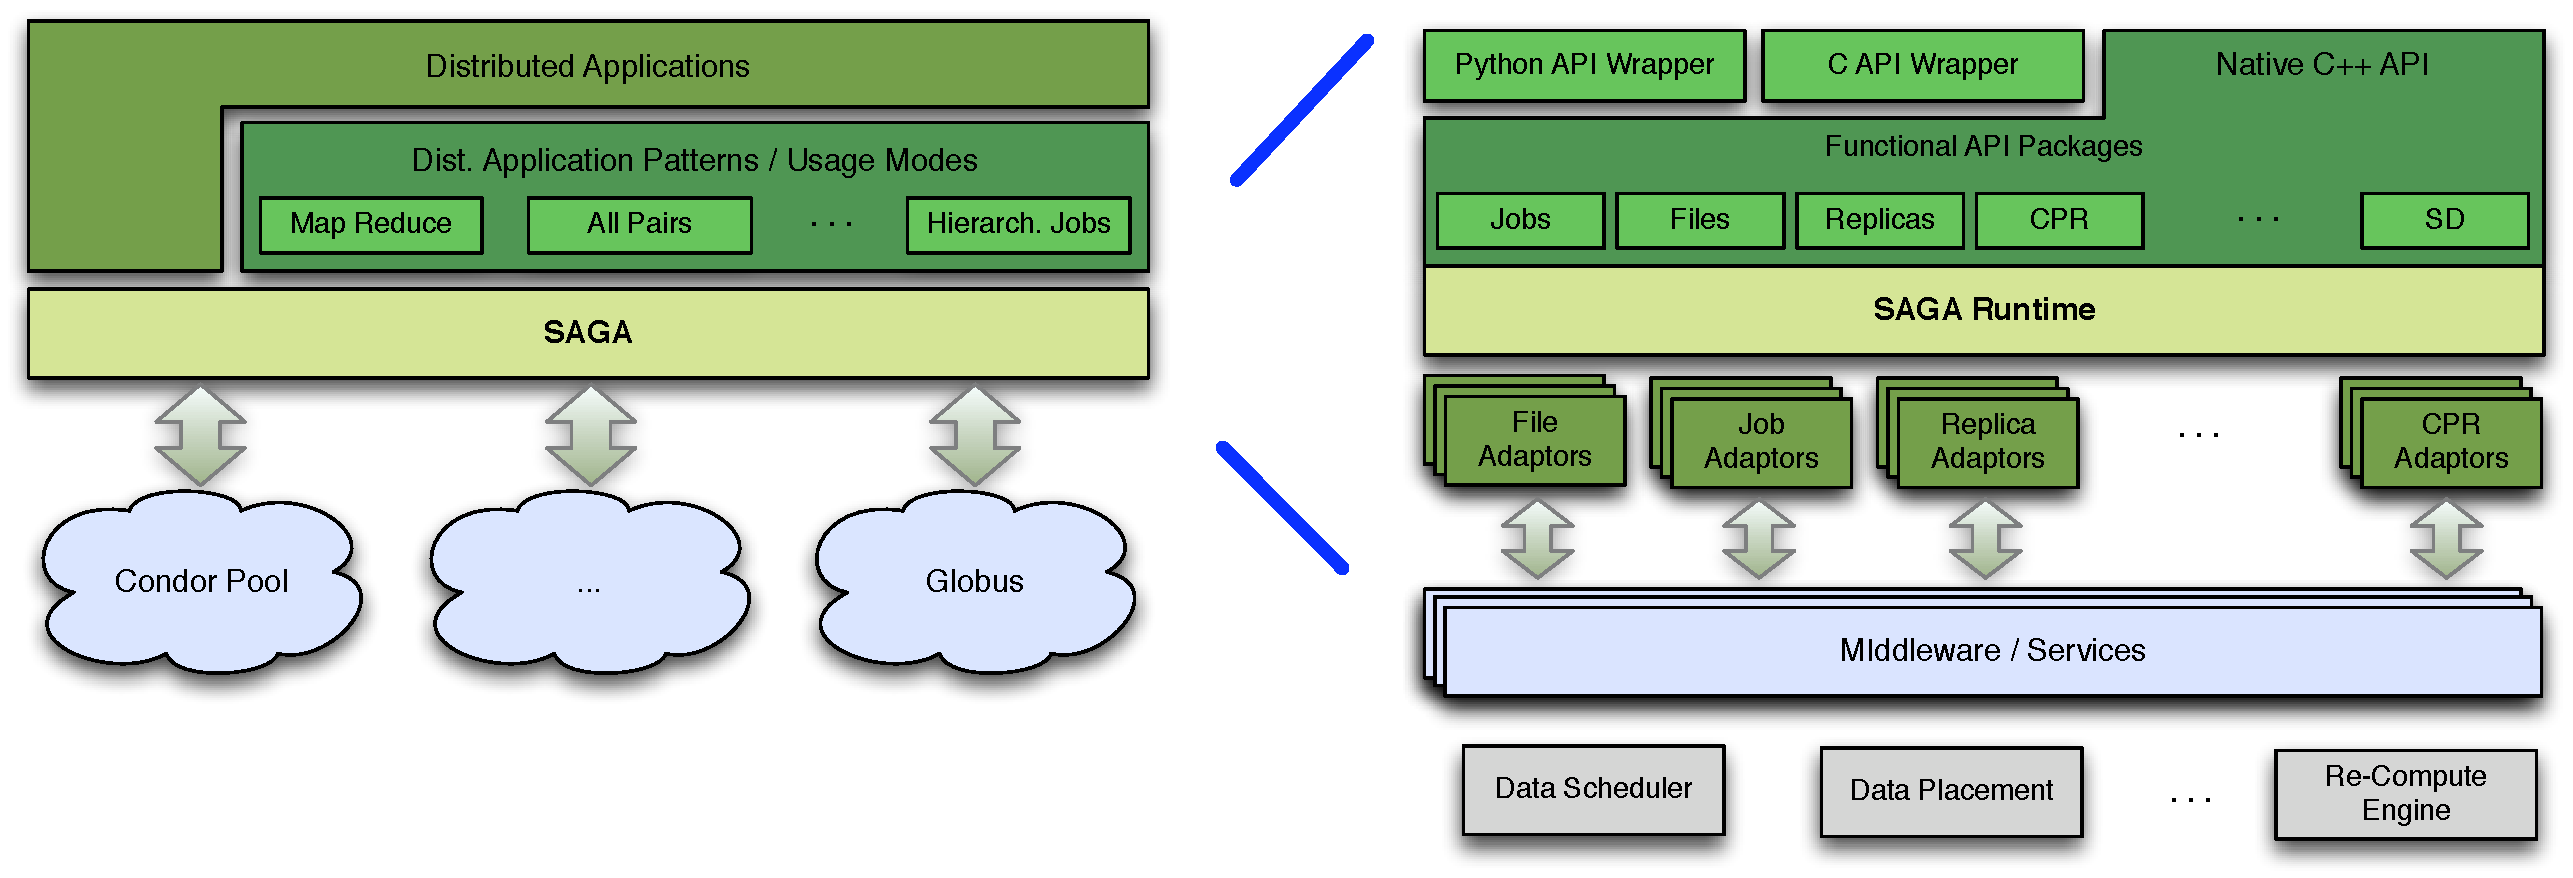
\includegraphics[width=\textwidth]{saga_comprehensive_2}}     
  \end{center}
  \caption{Schematic diagram showing how SAGA supports the development
    of three simple, but important ways of developing distributed
    applications. Layered schematic of the different components of the
    SAGA landscape. The core API supports the main functionality
    required by distributed applications.  Middleware specific
    adaptors make applications developed using SAGA grid portable.}
  \label{sagalayer}
\end{figure}
%\begin{itemize}

% \noindent Version 1.0~\cite{saga-core} of the specification has been submitted
% to the OGF editorial pipeline.  

\begin{compactitem}
\item File package - provides methods for accessing local and remote
  filesystems, browsing directories, moving, copying, and deleting
  files, setting access permissions, as well as zero-copy reading and
  writing. The replica package support the same functionality for logical files.
% \item Replica package - provides methods for replica management such
%   as browsing logical filesystems, moving, copying, deleting logical
%   entries, adding and removing physical files from a logical file
%   entry, and search logical files based on attribute sets.
\item Job package - provides methods for describing, submitting,
  monitoring, and controlling local and remote jobs. % Many parts of
%   this package were derived from the largely adopted
%   DRMAA~\cite{drmaa_url} specification.
\item Stream package - provides methods for authenticated local and
  remote socket connections with hooks to support authorization and
  encryption schemes.
\item RPC package - is an implementation of the OGF GridRPC
  API~\cite{gridrpc_url} definition and provides methods for unified
  remote procedure calls.
\end{compactitem}
%\end{itemize}

The SAGA Runtime Engine can dynamically load environment specific
adaptor (see Fig.~\ref{sagalayer}).  The two critical aspects of SAGA are its
{\it simplicity} of use and the fact that it is a proposed standard.
It is important to note, that these two properties provide the added
value of using SAGA for distributed application development.
Simplicity arises from being able to limit the scope to only the most
common and important grid-functionality required by applications.
Standardization represents the fact that the interface is derived from
a wide-range of applications using a collaborative approach and the
output of which is endorsed by the broader community.

\upp

\subsection{Developing Distributed Applications with SAGA}

\upp

SAGA can be used to develop and support distributed applications in
many different ways; the exact way in which it is used, in addition to
the application characteristics, depends upon factors such as how the
application needs to be used. For simplicity, in this paper, we will
discuss only three different approaches for distributed application
development (schematically summarized on the left side of
Fig.~\ref{sagalayer}).  First, applications can use SAGA directly for
standardised and simple distributed function calls that work on nearly
all middleware systems. Typically, applications developed using direct
SAGA calls are {\it explicitly} distributed.  Secondly, SAGA can be
used to create infrastructure independent frameworks (that support
patterns such as MapReduce), which provide distributed capability and
which can be used by applications to be {\it implicitly}
distributed. Thirdly, SAGA can be used to support usage modes that
provide access to distributed infrastructure, such as bulk
job-submission or hierarchical job-submission over different
machines. For this case too, applications are typically implicitly
distributed, and the knowledge/control of utilizing distributed
infrastructure is left to the SAGA-based framework that supports the
usage-mode. The RE application that we will discuss in the paper
belongs to the third category, whilst the EnKF based application is of
the first type.


\section{Applications With Loosely-Coupled Homogeneous
  Sub-Tasks: Replica-Exchange}  

\upp \alnote{Are we referring to sub-jobs as sub-tasks or sub-job? Just
  to keep this consistent with the other paper. We previously
  discussed that task has another meaning within SAGA, which could
  potentially lead to confusion.}
  
\jhanote{Andre, the word to avoid is ``tasks'', which is the term that
  has a SAGA specific context. I think we can safely use sub-tasks for
  sub-jobs if we like to. Especially given that the workshop is using
  a generic term -- ``multi-tasks''.}

% Replica-Exchange (RE) simulations~\cite{Sugita:1999rm},
% are an example of distributed applications consisting of homogeneous
% sub-tasks. 
RE~\cite{Sugita:1999rm} simulations can be used to understand
important physical phenomena -- ranging from protein folding dynamics
to binding affinity calculations required for computational drug
discovery.  For RE simulations utilizing as many distributed resources
as possible, is critical for the effective solution of the scientific
problem~\cite{repex_ptrsa}.  Distributed RE simulations must be able
to orchestrate different resources in a complex and dynamic
environment.  Writing such an applications is a complex task for a
myriad number of reasons~\cite{repex_escience08}. In the following a
SAGA-based RE framework developed for molecular dynamics simulations
is described.
% , not least of which is that distributed
% computing environments are inherently prone to
% failures

\upp

\subsection{Application Description}

\upp

% Replica-exchange simulations are also used to allow a sufficient
% sampling of configurations. This is an important requirement for
% connecting atomistic results to macroscopic or thermodynamic
% quantities available from experiments.  However, 

Even with the most powerful computing resources at the moment,
straight-forward Molecular Dynamics (MD) simulations are unable to
reach the relevant time-scales required to study conformational
changes and searches. This is partly due to the inherent limitations
in the MD algorithm -- a global synchronization is required at the end
of each time step.  This limitation provides an important motivation
for research into finding ways to accelerate sampling and enhance
``effective'' time-scales studied. Generalized ensemble approaches --
of which Replica-Exchange Molecular Dynamics
(REMD)~\cite{Sugita:1999rm} are a prominent example -- represent an
important and promising attempt to overcome the general limitations of
insufficient time-scales, as well as specific limitations of
inadequate conformational sampling arising from kinetic trappings.  In
the simplest formulation, RE is an algorithm whereby one
single long-running simulation is be substituted for an ensemble of
shorter-running similar simulations, but which are very
loosely-coupled, ie, the interval between exchange attempts is much
larger than the interval over which the simulations run; this also
make the RE formulation of physical problems excellent
candidates for distributed environments.

%\section{Replica Exchange Simulations}
% Replica Exchange simulations used within Molecular Dynamics (MD)
% approaches,

\upp

\subsection{Application Architecture}

\upp

There are many architectural aspects of the framework used to
implement RE simulations. However, we will focus on the abstractions
that we create using SAGA that enable efficient job-submission on any
underlying infrastructure.  Details of the architecture and
abstractions can be found in
Ref.~\cite{repex_ptrsa,repex_escience08}. Here we present the
architecture in the context of an application consisting of
loosely-coupled multiple sub-tasks. RE simulations can be thought of
as consisting of two distinct components: the simulation
engine/mechanism used for each replica process, and the
orchestration-coupling mechanism between the individual replicas. Our
current RE framework uses NAMD for the former and a SAGA-based
framework for orchestration and coordination of the replica sub-tasks.

The developed RE framework~\cite{repex_escience08} comprises of the
\emph{RE-Manager} -- the central master deployed on the user's
desktop, and the \textit{Replica-Agents}, that reside on the machines
where RE simulations are carried out. The RE-Manager orchestrates all
replicas, i.\,e.\ it is responsible for the parameterization of
replica tasks, file staging, job spawning and the conduction of the
replica-exchange itself.  The Replica-Agent is responsible for
spawning and monitoring the sub-tasks.

In particular, queueing delays can represent a major bottleneck: a
single crowded resource can slowdown the simulation arbitrary. Thus,
to achieve an optimal time to solution, RE sub-tasks need to be
dispatched efficiently.  A common principle to prevent this is the
usage of Glide-In jobs, which represent a placeholder for a set of
sub-tasks (see Ref.~\cite{citeulike:291860}).  For a Glide-In
job, a sufficiently large chunk of resources is requested. Smaller
sub-tasks can then rapidly be executed through the Glide-In job.
Figure~\ref{fig:remdmanager_v11} summarizes the abstractions used
within the RE framework.

\begin{figure}[htbp]
    \centering
        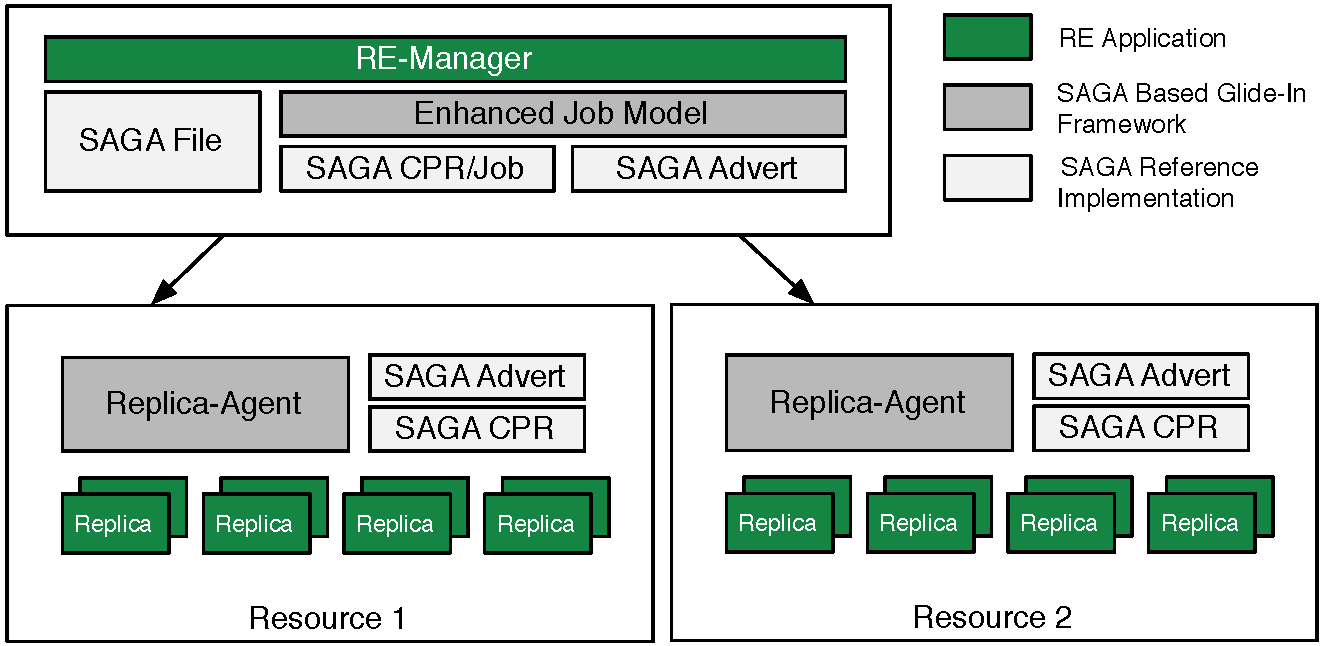
\includegraphics[width=4.5in]{remdmanager_v11.pdf}
        \caption{Replica Exchange Framework Abstractions: The
          Replica-Agent is used as placeholder job for all sub-tasks
          running on a single cluster. The RE-Manager can control both
          the Replica-Agents and the replica jobs using a SAGA-based
          user-level job API. By using this efficient way to allocate
          resources, queuing times are minimized and the time to
          completion can be dramatically reduced when using multiple
          and single resources. \up}
    \label{fig:remdmanager_v11}
\end{figure}  
% The SAGA Glide-In framework comprises of two components: 1) The
% Glide-In manager provides the enhance job model API and allows the
% management of both Glide-In jobs and sub-tasks.  2) The Replica-Agents
% represent the Glide-In jobs. The agents manage their allocated
% resources and dispatch sub-tasks on request. In this sense the
% Replica-Agents implement the functionality of an application-level
% scheduler. Communication between the Replica-Agent and Glide-In
% manager is carried out using the SAGA advert service, a central
% key/value store.

% With this capability the SAGA Glide-In framework provides a novel
% system-level abstraction for allocating larger chunks of resources and
% for mapping these resources to a set of sub-jobs.%  The enhanced job
% % model can be used as drop-in replacement for SAGA job objects.
% No code modification is required -- the application only maps the
% sub-tasks to a suitable Glide-In job.  The RE-Manager relies on the
% SAGA Glide-In framework to reserve resources on a cluster and to
% efficiently dispatch RE processes to these nodes.

While the implementation of the enhanced job model is entirely based
on SAGA %and in particular the SAGA Advert Service,
we can utilise other frameworks, such as the original Condor
Glide-In~\cite{citeulike:291860}. % or Falcon~\cite{1362680}.
Currently, we are actively working on a Condor adaptor for
SAGA~\cite{saga_condor_url}, which will also support native Glide-In
functionality for Condor Jobs; our enhanced job model will then serve
as abstraction, while the Condor level Glide-In will be used where
appropriate.  Irrespective of that, however, the strengths of our
approach are the following: A general purpose Glide-in mechanism that
does not require either Condor, or Globus and in which sub-tasks are
part of a Glide-In meta-job, can be controlled at the
application-level using simple {\it ssh} if needed. Secondly, the same
mechanisms can be used to exploit distributed
resources~\cite{repex_ptrsa}, as well as single high-end resources,
without any changes in application code.  This represents the basis of
our claim of independence from underlying-infrastructure.

\up

\subsection{Application Deployment}

\up

% To evaluate the feasibility and performance of the RE-Manager several
% experiments have been conducted on the TeraGrid~\cite{teragrid} and
% LONI~\cite{loni}.  

We have shown how using the SAGA Glide-In infrastructure on multiple
TeraGrid/LONI resources, the time-to-solution can be
reduced~\cite{Luckow:2008la}. Continuing with the theme that well
developed abstractions can serve across the spectrum -- distributed
HPC machines (such as the TeraGrid) to single high-end supercomputers
(such as Abe or QueenBee) to many smaller machines flocked together
(Condor style high-throughput), we focus on using the same
infrastructure to reduce the time-to-solution on a single machine.
This is also a test of the scalability of the SAGA-based Glide-In
framework on a single machines. % (QueenBee (QB)).

Figure~\ref{perf_remd_glidin} shows that the Glide-In framework is
especially beneficial if there are fluctuations in the queue-time for
the sub-tasks (which is almost always!). The more sub-tasks are
spawned, the more likely such delays become. While with
the SAGA Glide-In framework the runtime only modestly increase with
more than 8 replicas, the runtime rapidly rises when using regular
Globus job for spawning NAMD tasks. The unpredictable nature of these
queueing times becomes obvious by the high standard deviation found in
the measurements.

\begin{figure}[htbp]
  \subfigure{\label{perf_remd_glidin} 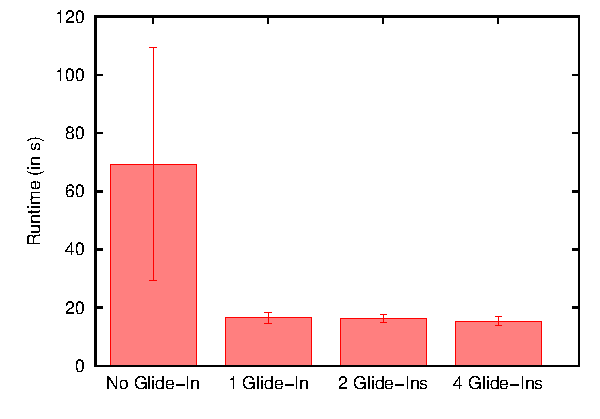
\includegraphics[width=0.5\textwidth]{perf_glidein.pdf}}
  \subfigure{\label{exchange-165} 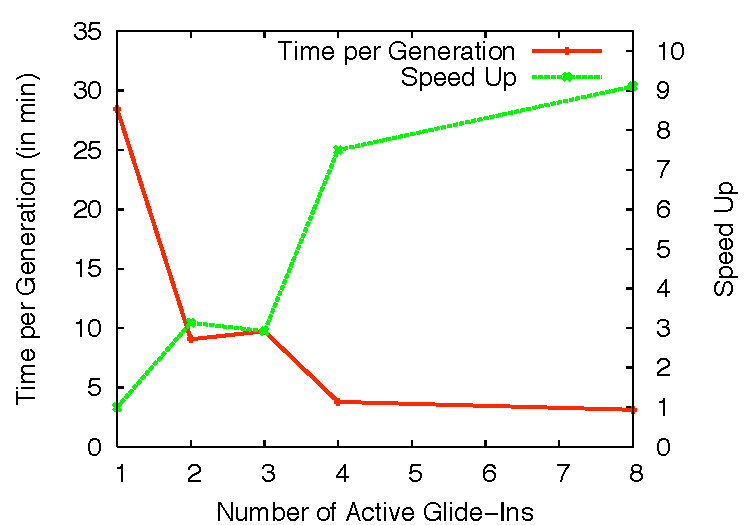
\includegraphics[width=0.5\textwidth]{perf_repex2.pdf}}
  \caption{SAGA Glide-In Performance: The figure shows the average
    runtime of a RE simulation with 16 RE processes running on 16
    cores each on QueenBee.  The Glide-In framework provides the
    possibility to effectively cluster RE jobs to receive a
    significant reduced time to solution (upto
    80\,\%) even on a single machine.
    % (1) The plots show the time-series of the average times between
%     exchange attempts (in red and using the left-hand y axis) and 
    The plot on the right shows the number of active Glide-Ins over a
    six-hour run on the TeraGrid.  The plot in red (using the
    left-hand y axis) illustrates how the average time between
    exchange attempts (inverse of physical efficiency) decreases as
    the number of Glide-Ins increases. The plot in green shows the
    speedup.}
\end{figure}

Figure~\ref{perf_remd_glidin} shows that the SAGA Glide-In framework
can provide a reduced time to solution even on a single machine by
avoiding queuing time delays and fluctuations for every sub-task and
allowing the efficient dispatching of RE tasks solely through the
Replica-Agent. During our experiments we were able to measure speedups
of up to 80\,\% compared to the non Glide-In
approach. Fig.~\ref{exchange-165} shows several measures of how the
use of SAGA framework results in efficient and effective deployment.

% The unpredictable nature of these queueing times is reflected in the
% high standard deviation observed in the runtimes. While queueing times
% also have an impact on Glide-Ins, these are in general less severe.
% Further, for the Glide-In scenario, the queueing times become
% negligible, the longer the RE simulation is (the runtimes have been
% kept short for this simple scenario). In contrast, when no Glide-Ins
% are used every sub-jobs is subject to the queuing delay at the local
% scheduler.

% The SAGA Glide-In framework can efficiently dispatch RE sub-tasks
% providing an enhanced time to solution even when deployed on a single
% machines. 2) By using a clever assignment of Glide-Ins to hosts and
% jobs, the runtime can be further optimized. In future, we plan to
% utilize this by deploying adaptive optimization strategies at runtime.

% By avoiding long queuing time for big jobs, a distribution of the
% replica processes to a set of less crowded resources provides a lot of
% benefits.

% In certain situation the usage of smaller jobs can have an advantage,
% e.\,g.\ when the local scheduler backfills such jobs. However, usually
% not all replica processes can be backfilled -- the more processes are
% spawned the more likely are delays.

% The framework has also been deployed on multiple resources
% concurrently. This is in particular useful for smaller resources, such
% as Oliver, where it is only possible to request 64 cores at a time. In
% contrast to the QB only run, the runtime only slightly increases by
% about 1.5 minutes, which is acceptable compared to a possible delay
% due to insufficient resources on Poseidon.




\section{Loosely-Coupled Heterogeneous Sub-Tasks: Kalman-Filter
  Simulations}

\upp

Ensemble Kalman filters (EnKF) are widely used in science and
engineering~\cite{KalmanPaper}.  EnKF are recursive filters that can
be used to handle large, noisy data. The data can be the set of
results and parameters of ensembles of different models of a
particular physical system. The ensembles are run through the KF to
obtain the true physical state of the data ~\cite{KalmanPaper}, to
effectively solve the inverse problem.

\upp

\subsection{Application Description}

% \subsection{SAGA and Cactus: A Powerful Application Development
%   Framework}
% \subsection{Deploying on Distributed Resources}
% \subsection{Deploying on Abe}
% BQP used for the first time to dynamically determine queue and model
% size within a given system to submit sub-task to...
%\section{}

\upp

In EnKF, an ensemble of forward models are run with different
parameters. The data they produce is assimilated at the end of each
stage, the parameters are corrected, and the models are run
again. This process is repeated several times until a pre-determined
criteria has been met. The ensemble of forward models are run as
sub-tasks on possibly different machines, launched by a master filter
task using SAGA. SAGA is also used to control the flow of data between
the filter and the ensemble of models.

% \begin{figure}[htbp]
%     \centering
%     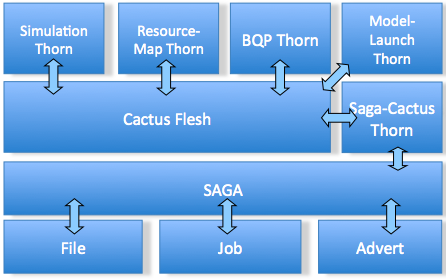
\includegraphics[width=0.44\textwidth]{kalmanfilterlayer.png}
%     \caption{Layered Diagram of the various components of the EnKF
%       application. Each sub-task is a malleable application --
%       checkpoint and restart ready on different number of processor;
%       many of these capabilities are provided by Cactus.  SAGA is used
%       to provide control of the required distributed functionality --
%       identifying best resource for sub-tasks, submitting these
%       sub-tasks etc. See Ref~\cite{saga_tg08} for more details.\up\up}
%     \label{fig:kalmanfilter}
% \end{figure}  

The variation in model parameters often has a direct and sizable
influence on the complexity of solving the underlying equations, thus
varying the required runtime of different models.  
% The end-to-end application consists of several stages; in general at
% each stage the number of models generated varies (each model is solved
% via a sub-task). The size and granularity of the models also varied
% within a stage; consequently for any given stage, the resource
% requirements of each sub-task varied (from 4 processors to 64
% processors). The run-time of each model was unpredictable and
% uncorrelated with the run-time of models running on the same number of
% processors – a truly independent variable.  This is the fundamental
% reason behind the fact that the individual sub-tasks are heterogeneous
% with varying run-times and resource requirements (if not very
% hard-to-predict). 
Since we need both parameters and results for the
EnKF, a mechanism to assign models to available resources based on
their expected time to completion and resource requirement is useful.
Such a mechanism estimates the time a model will spend in the queue of
a resource, the time it needs to run, and the time required to migrate
the data it requires/produces back and forth, and based on that
attempt to minimize the time required to perform each Kalman filter
iteration.  In fact, with changing resource simulation requirements
(as is the case with models that find themselves lagging behind the
rest of the model pack), a mechanism which can take advantage of
faster, cheaper or more powerful machines is even more
advantageous~\cite{escience07}.

We have developed a mechanism whereby EnKF can be solved using
multiple-resources, using application-level scheduling applied
dynamically~\cite{saga_tg08}, ie mapping the sub-tasks requirement to
the resources available at the instant the sub-tasks become available
and ready to run, as opposed to {\it a priori} static method of job
submission.  For the problem size studied, the sub-tasks required
mostly less than 32 processors. For this paper we used the earlier
developed frameworks and deployed it on a single large machine --
NCSA's Abe~\footnote{We wanted to use Ranger, but BQP was not
  available on Ranger, and would not have been before the submission
  of this paper}. %  For small physical models where sub-tasks are
% typically small -- both spatially and temporally, overheads in using
% multiple, distributed machines most often result in total
% time-to-solution being higher than if a large monolithic
% single-machine were used. But as shown in
% Ref~\cite{novelsubmissionmode}, as the number of processors requested
% for a sub-task increases, the total wait time in the queueing system,
% often goes up (disproportionately). Thus
A mechanism (multiple, distributed versus single machine) that is more
efficient for physical models with sub-tasks that have typically low
processor counts, will not necessarily be the more efficient as the
typical sub-task size increases. Therefore it is crucial that any
general-purpose solution be usable on both single large machines to
multiple machines.  \jhanote{Yaakoub, do you have measure of
  time-to-completion for the two-cases of the toy-problem?}  We can
enhance throughput further by applying the Glide-In mechanisms
discussed in the earlier section, which facilitate dynamic tasks being
aggregated from similar sub-tasks. We will report on the results of
this and whether the framework can be used on high-end petascale
supercomputers in future work.

%that to determine the best resource to use at

While concurrently running on various machines is advantageous by
simple virtue of the fact that more resources would be available for
running the forward models, it is also more technically challenging
than running on a single machine.  Authentication, job launching,
multiple executables in correct paths for different architectures and
file systems, and of course file transfer across the different
machines are all possible points of failure. % Rigorous fault tolerance
% can be built into application framework using
% SAGA~\cite{Luckow:2008la}.
These are just some of the additional reasons why a high-level
interface such as SAGA is required to hide the heterogeneity of
different distributed systems. In spite of that, several challenges
remain -- technical, sociological as well as policy level, some
specific examples of relevance we discuss in the next section.

% It can be argued that running all the models on a single large machine
% would be a simpler solution as the afore-mentioned technical
% difficulties; however a new range of challenges emerge. We are

\up

\section{Deploying on Distributed Resources}

\up

\jhanote{Yaakoub/Andre: We need a paragraph about the problems that we
  faced in getting SAGA working on Ranger and why ultimately we were
  unable to get through} \alnote{Added some remarks regarding the
  Globus problems.}

As mentioned in the opening section, using SAGA we have developed
programming and execution models, whereby applications are independent
of the underlying infrastructure, i.e., either use a monolithic
mammoth machine, or multiple-distributed machines, depending upon the
physical problem being investigated, without any modification at the
application-level code. In spite of these theoretical advances, in
practise end-users often find it more convenient to use single
resources, even if not optimally-efficient.  The smooth and effective
deployment of distributed applications on heterogeneous resources
remains is a difficult task.  To highlight just some of the challenges
of deploying advanced application on general-purpose distributed
infrastructure, we mention the fact that at best 33\% of the resources
we tried were usable (ie two in three were not usable) .  We mention
two problems that we encountered and led to a high amount of
complexity: different library versions and broken Globus
installations.  Also, Globus installations on TeraGrid machines proved
to be quite different.  For example, the Globus GRAM2 versions on Abe
and QueenBee map the RSL count element different: While on QB the
count element is mapped to the number of cores, on Abe this element
describes the number of nodes. Further standardization of this aspect
is required in the future. The GRAM2 on Ranger (in particular the Sun
GridEngine adaptor) was completely unusable due to the lack of support
for MPI jobs.

% To evaluate the performance of the REMD-Manager several experiments
% have been conducted on the TeraGrid~\cite{teragrid} and
% LONI~\cite{loni}. The RE-Manager has been extensively tested on
% QueenBee (QB) using 16 replica processes, a total of 256 cores.  The
% RE processes have been distributed to a variable number of Glide-In
% jobs.

Deploying our applications on ranger was not a straightforward task.
SAGA requires a recent installation of the BOOST library which we had
to compile ourselves. When we were finished compiling our
applications, we ran into a job submission problem on a particular
login node. %After the node was rebooted, we discovered there was an an
%issue with the globus installation. 
Moving past the firewall and GRAM2 issues, getting the right
certificates that are recognized on the machine, we discovered there
were even more issues that need to be resolved: GridFTP was not
working, the Globus/SGE script had a small error in it that had to be
corrected.  These issues are outlined in tickets 4957, 5111, 5130,
5145, 5172 and 5174. It is important to note that we encountered
excellent response time and expert system administrators who resolved
all of these issues promptly, but reiterates the complexity of
utilising multiple resources from general-purpose grids.  The aim here
is not to criticise any provider -- resource or software product, but
to simply highlight the practical challenges of deploying distributed
applications.

%\jhanote{Will need to shorten this paragraph}


% The more processes are spawned, the more likely are such
% delays. While with the SAGA Glide-In framework the runtime only
% modestly increase with more than 8 replicas, the runtime rapidly
% rises when using regular Globus job for spawning NAMD tasks.  By
% avoiding long queuing time for big jobs, a distribution of the
% replica processes to a set of less crowded resources provides a lot
% of benefits.

\up\upp

\section{Conclusions and Discussions}

\upp

SAGA provides the abstractions and the ability to create applications
with multiple sub-tasks that can exploit multiple and different
infrastructure types.  We have demonstrated this via the
implementation of two distinct, specific applications but both
representative of a broader class of applications and running them in
two different execution environments without changing the application
in any way! The specific applications differed not only in the types
of sub-tasks (homogeneous versus heterogeneous) but also in the nature
of the coupling between the sub-tasks.
  
\jhanote{not sure what to do with this: Not only do we need support
  for different programming models, this is also proof of support for
  agile execution models.}

It is interesting to note that {\it simple, naive} implementations of
these applications are possible; these would require these
applications to be ``grid-unaware'' (or implicitly distributed).
Although we don't provide details here, the real power of these
applications arise from their ability to have an agile execution
model, i.e., by being adaptive to dynamic resource requirements or
availability. In other words, in order to develop applications that
have agile execution models, more often than not, applications need to
explicitly control the distributed aspects, i.e., be {\it grid-aware}
We posit that SAGA provides an important mechanism to develop
explicitly distributed applications.

% We believe explicit control is a critical for adaptive applications
% and posit that SAGA provides an important mechanism to implement the
% distributed features explicitly.

% Finally, somewhat related to the concept of explicitly distributed
% applications, is the challenge of optimally scheduling sub-tasks.
Optimal scheduling of sub-tasks remains a challenge of distributed
computing; however as demonstrated, for adaptive applications,
scheduling can often be done effectively at the application level.
This is possible because, as shown, adaptive applications don't
necessarily need tight co-scheduling, but often just
lightweight-coupling between resources. This is yet another advantage
of an agile-execution model.

\jhanote{Conclude with the note that the same development framework can be
used on a single high-end computer.}

\jhanote{Need to talk about algorithms that can be decomposed
  spatially, but retain a level of synchronisation, between stages,
  There is a challenge in the scheduling of the sub-tasks.  This is
  probably a general challenge/problem of ``many tasks'' computing;
  there isn't always a need for tight co-scheduling, but a need for
  some level of loose coupled scheduling.  Some level of best effort
  resource allocation is acceptable.}

\up\upp

\section*{Acknowledgement}

\upp

Important funding for SAGA specification and development has been
provided by the UK EPSRC grant number GR/D0766171/1.  SJ also
acknowledges the e-Science Institute, Edinburgh for supporting the
research theme, ``Distributed Programming Abstractions''. This work
would not have been possible without the efforts and support of the
wider SAGA team. This work has also been made possible thanks to the
internal resources of the Center for Computation \& Technology (CCT)
at Louisiana State University and computer resources provided by LONI.

\up\upp

\bibliographystyle{splncs}
\bibliography{saga,literatur}

\end{document}





% \Section{Introduction}
%   There exist several applications which require several smaller but
%   heterogenous tasks to be solved in multiple-stages as part of the
%   overall solution.  Often the time-to-solution is the single most
%   important metric.  Distributed resources can thus help, especially
%   when combined with opportunistic scheduling/execution.  However, the
%   desire/need to use distributed computing comes with its own/unique
%   set of challenges.
  
%   We discuss three application types that are in turn composed of
%   multiple, smaller but {\it loosely-coupled} tasks -- Replica
%   Dynamics, Satisfiability problems, and Kalman filtering
%   applications.  Although these applications types are similar in that
%   they are comprised of multiple, smaller tasks, they are different in
%   that the individual sub-tasks are dissimilar for different reasons.
  
%   These application types are often multi-staged, with varying levels
%   of dependency between the stages. There could be, strict ordering
%   between the stages, ie. if all tasks in a stage must complete and be
%   globally synchronised before the next stage can begin. Thus there is
%   coupling between tasks within a given stage, and there is coupling
%   between stages.

%   Other challenges that any many-task system will encounter are: (i)
%   scheduling these sub-tasks is a challenge, (ii) level of speculative
%   computing that can be employed.

%   In parallel replica dynamics, the replicas can run for different
%   time durations between different stages. In replica-exchange
%   dynamics, the number and frequency of exchanges can vary.  Different
%   stages of this application vary; in other words, there is
%   time-domain heterogenity.

%   In Kalman filter based applications, the number and size of 
%   tasks between different stages varies. 

%   In the general class of satisfiability-based applications, as well
%   as the learning-based algorithms, there are elements of both kinds
%   of heterogenity between stages. GridSAT is an interesting example.
         
%\newpage


